% Created by tikzDevice version 0.12.3 on 2020-05-14 20:48:40
% !TEX encoding = UTF-8 Unicode
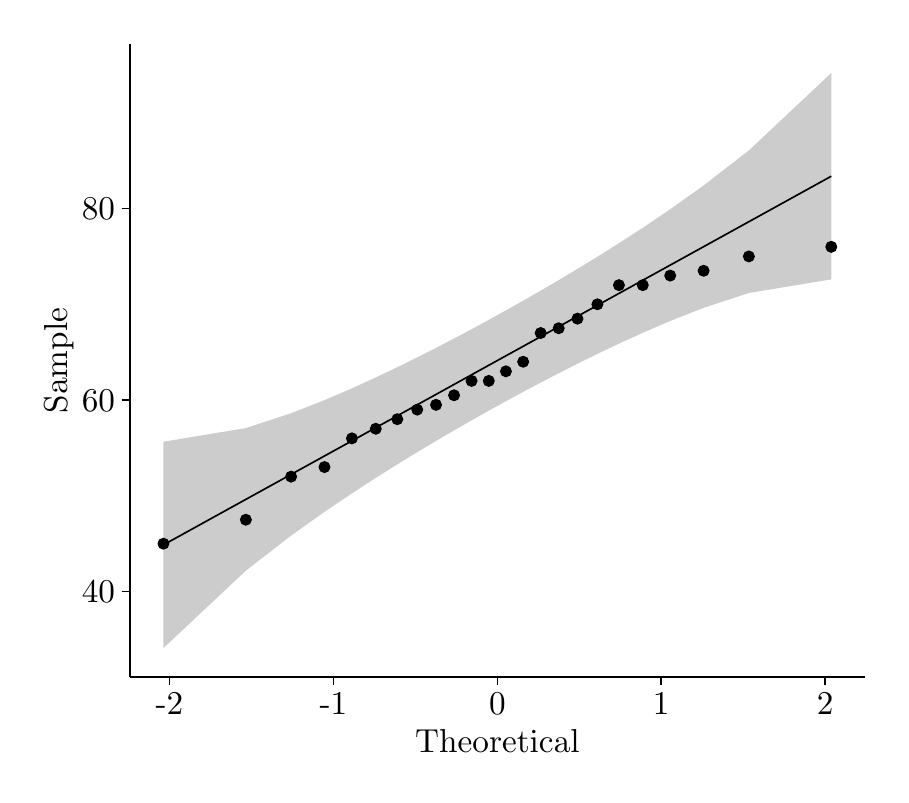
\begin{tikzpicture}[x=1pt,y=1pt]
\definecolor{fillColor}{RGB}{255,255,255}
\path[use as bounding box,fill=fillColor,fill opacity=0.00] (0,0) rectangle (308.44,270.16);
\begin{scope}
\path[clip] (  0.00,  0.00) rectangle (308.44,270.16);
\definecolor{drawColor}{RGB}{255,255,255}
\definecolor{fillColor}{RGB}{255,255,255}

\path[draw=drawColor,line width= 0.6pt,line join=round,line cap=round,fill=fillColor] (  0.00,  0.00) rectangle (308.44,270.16);
\end{scope}
\begin{scope}
\path[clip] ( 36.99, 35.59) rectangle (302.44,264.16);
\definecolor{fillColor}{RGB}{255,255,255}

\path[fill=fillColor] ( 36.99, 35.59) rectangle (302.44,264.16);
\definecolor{drawColor}{RGB}{0,0,0}
\definecolor{fillColor}{RGB}{0,0,0}

\path[draw=drawColor,line width= 0.4pt,line join=round,line cap=round,fill=fillColor] ( 49.06, 83.70) circle (  1.96);

\path[draw=drawColor,line width= 0.4pt,line join=round,line cap=round,fill=fillColor] ( 78.84, 92.35) circle (  1.96);

\path[draw=drawColor,line width= 0.4pt,line join=round,line cap=round,fill=fillColor] ( 95.19,107.92) circle (  1.96);

\path[draw=drawColor,line width= 0.4pt,line join=round,line cap=round,fill=fillColor] (107.25,111.38) circle (  1.96);

\path[draw=drawColor,line width= 0.4pt,line join=round,line cap=round,fill=fillColor] (117.17,121.76) circle (  1.96);

\path[draw=drawColor,line width= 0.4pt,line join=round,line cap=round,fill=fillColor] (125.79,125.22) circle (  1.96);

\path[draw=drawColor,line width= 0.4pt,line join=round,line cap=round,fill=fillColor] (133.57,128.68) circle (  1.96);

\path[draw=drawColor,line width= 0.4pt,line join=round,line cap=round,fill=fillColor] (140.76,132.14) circle (  1.96);

\path[draw=drawColor,line width= 0.4pt,line join=round,line cap=round,fill=fillColor] (147.56,133.87) circle (  1.96);

\path[draw=drawColor,line width= 0.4pt,line join=round,line cap=round,fill=fillColor] (154.07,137.33) circle (  1.96);

\path[draw=drawColor,line width= 0.4pt,line join=round,line cap=round,fill=fillColor] (160.40,142.52) circle (  1.96);

\path[draw=drawColor,line width= 0.4pt,line join=round,line cap=round,fill=fillColor] (166.62,142.52) circle (  1.96);

\path[draw=drawColor,line width= 0.4pt,line join=round,line cap=round,fill=fillColor] (172.81,145.98) circle (  1.96);

\path[draw=drawColor,line width= 0.4pt,line join=round,line cap=round,fill=fillColor] (179.04,149.44) circle (  1.96);

\path[draw=drawColor,line width= 0.4pt,line join=round,line cap=round,fill=fillColor] (185.37,159.82) circle (  1.96);

\path[draw=drawColor,line width= 0.4pt,line join=round,line cap=round,fill=fillColor] (191.88,161.55) circle (  1.96);

\path[draw=drawColor,line width= 0.4pt,line join=round,line cap=round,fill=fillColor] (198.67,165.01) circle (  1.96);

\path[draw=drawColor,line width= 0.4pt,line join=round,line cap=round,fill=fillColor] (205.87,170.20) circle (  1.96);

\path[draw=drawColor,line width= 0.4pt,line join=round,line cap=round,fill=fillColor] (213.65,177.12) circle (  1.96);

\path[draw=drawColor,line width= 0.4pt,line join=round,line cap=round,fill=fillColor] (222.27,177.12) circle (  1.96);

\path[draw=drawColor,line width= 0.4pt,line join=round,line cap=round,fill=fillColor] (232.18,180.58) circle (  1.96);

\path[draw=drawColor,line width= 0.4pt,line join=round,line cap=round,fill=fillColor] (244.25,182.31) circle (  1.96);

\path[draw=drawColor,line width= 0.4pt,line join=round,line cap=round,fill=fillColor] (260.60,187.50) circle (  1.96);

\path[draw=drawColor,line width= 0.4pt,line join=round,line cap=round,fill=fillColor] (290.38,190.96) circle (  1.96);

\path[draw=drawColor,line width= 0.6pt,line join=round] ( 49.06, 83.27) --
	( 78.84, 99.71) --
	( 95.19,108.73) --
	(107.25,115.39) --
	(117.17,120.86) --
	(125.79,125.62) --
	(133.57,129.92) --
	(140.76,133.89) --
	(147.56,137.64) --
	(154.07,141.24) --
	(160.40,144.73) --
	(166.62,148.17) --
	(172.81,151.58) --
	(179.04,155.02) --
	(185.37,158.51) --
	(191.88,162.11) --
	(198.67,165.86) --
	(205.87,169.83) --
	(213.65,174.13) --
	(222.27,178.89) --
	(232.18,184.36) --
	(244.25,191.02) --
	(260.60,200.04) --
	(290.38,216.48);
\definecolor{fillColor}{RGB}{0,0,0}

\path[fill=fillColor,fill opacity=0.20] ( 49.06,120.55) --
	( 78.84,125.46) --
	( 95.19,130.84) --
	(107.25,135.57) --
	(117.17,139.84) --
	(125.79,143.77) --
	(133.57,147.47) --
	(140.76,151.02) --
	(147.56,154.46) --
	(154.07,157.84) --
	(160.40,161.20) --
	(166.62,164.57) --
	(172.81,167.99) --
	(179.04,171.49) --
	(185.37,175.12) --
	(191.88,178.93) --
	(198.67,182.99) --
	(205.87,187.39) --
	(213.65,192.27) --
	(222.27,197.86) --
	(232.18,204.54) --
	(244.25,213.13) --
	(260.60,225.80) --
	(290.38,253.77) --
	(290.38,179.20) --
	(260.60,174.29) --
	(244.25,168.91) --
	(232.18,164.18) --
	(222.27,159.91) --
	(213.65,155.98) --
	(205.87,152.28) --
	(198.67,148.73) --
	(191.88,145.29) --
	(185.37,141.91) --
	(179.04,138.55) --
	(172.81,135.18) --
	(166.62,131.76) --
	(160.40,128.26) --
	(154.07,124.63) --
	(147.56,120.82) --
	(140.76,116.76) --
	(133.57,112.36) --
	(125.79,107.48) --
	(117.17,101.89) --
	(107.25, 95.21) --
	( 95.19, 86.62) --
	( 78.84, 73.95) --
	( 49.06, 45.98) --
	cycle;

\path[] ( 49.06,120.55) --
	( 78.84,125.46) --
	( 95.19,130.84) --
	(107.25,135.57) --
	(117.17,139.84) --
	(125.79,143.77) --
	(133.57,147.47) --
	(140.76,151.02) --
	(147.56,154.46) --
	(154.07,157.84) --
	(160.40,161.20) --
	(166.62,164.57) --
	(172.81,167.99) --
	(179.04,171.49) --
	(185.37,175.12) --
	(191.88,178.93) --
	(198.67,182.99) --
	(205.87,187.39) --
	(213.65,192.27) --
	(222.27,197.86) --
	(232.18,204.54) --
	(244.25,213.13) --
	(260.60,225.80) --
	(290.38,253.77);

\path[] (290.38,179.20) --
	(260.60,174.29) --
	(244.25,168.91) --
	(232.18,164.18) --
	(222.27,159.91) --
	(213.65,155.98) --
	(205.87,152.28) --
	(198.67,148.73) --
	(191.88,145.29) --
	(185.37,141.91) --
	(179.04,138.55) --
	(172.81,135.18) --
	(166.62,131.76) --
	(160.40,128.26) --
	(154.07,124.63) --
	(147.56,120.82) --
	(140.76,116.76) --
	(133.57,112.36) --
	(125.79,107.48) --
	(117.17,101.89) --
	(107.25, 95.21) --
	( 95.19, 86.62) --
	( 78.84, 73.95) --
	( 49.06, 45.98);
\end{scope}
\begin{scope}
\path[clip] (  0.00,  0.00) rectangle (308.44,270.16);
\definecolor{drawColor}{RGB}{0,0,0}

\path[draw=drawColor,line width= 0.6pt,line join=round] ( 36.99, 35.59) --
	( 36.99,264.16);
\end{scope}
\begin{scope}
\path[clip] (  0.00,  0.00) rectangle (308.44,270.16);
\definecolor{drawColor}{RGB}{0,0,0}

\node[text=drawColor,anchor=base east,inner sep=0pt, outer sep=0pt, scale=  1.20] at ( 31.59, 62.27) {40};

\node[text=drawColor,anchor=base east,inner sep=0pt, outer sep=0pt, scale=  1.20] at ( 31.59,131.47) {60};

\node[text=drawColor,anchor=base east,inner sep=0pt, outer sep=0pt, scale=  1.20] at ( 31.59,200.67) {80};
\end{scope}
\begin{scope}
\path[clip] (  0.00,  0.00) rectangle (308.44,270.16);
\definecolor{drawColor}{RGB}{0,0,0}

\path[draw=drawColor,line width= 0.6pt,line join=round] ( 33.99, 66.40) --
	( 36.99, 66.40);

\path[draw=drawColor,line width= 0.6pt,line join=round] ( 33.99,135.60) --
	( 36.99,135.60);

\path[draw=drawColor,line width= 0.6pt,line join=round] ( 33.99,204.80) --
	( 36.99,204.80);
\end{scope}
\begin{scope}
\path[clip] (  0.00,  0.00) rectangle (308.44,270.16);
\definecolor{drawColor}{RGB}{0,0,0}

\path[draw=drawColor,line width= 0.6pt,line join=round] ( 36.99, 35.59) --
	(302.44, 35.59);
\end{scope}
\begin{scope}
\path[clip] (  0.00,  0.00) rectangle (308.44,270.16);
\definecolor{drawColor}{RGB}{0,0,0}

\path[draw=drawColor,line width= 0.6pt,line join=round] ( 51.24, 32.59) --
	( 51.24, 35.59);

\path[draw=drawColor,line width= 0.6pt,line join=round] (110.48, 32.59) --
	(110.48, 35.59);

\path[draw=drawColor,line width= 0.6pt,line join=round] (169.72, 32.59) --
	(169.72, 35.59);

\path[draw=drawColor,line width= 0.6pt,line join=round] (228.96, 32.59) --
	(228.96, 35.59);

\path[draw=drawColor,line width= 0.6pt,line join=round] (288.19, 32.59) --
	(288.19, 35.59);
\end{scope}
\begin{scope}
\path[clip] (  0.00,  0.00) rectangle (308.44,270.16);
\definecolor{drawColor}{RGB}{0,0,0}

\node[text=drawColor,anchor=base,inner sep=0pt, outer sep=0pt, scale=  1.20] at ( 51.24, 21.93) {-2};

\node[text=drawColor,anchor=base,inner sep=0pt, outer sep=0pt, scale=  1.20] at (110.48, 21.93) {-1};

\node[text=drawColor,anchor=base,inner sep=0pt, outer sep=0pt, scale=  1.20] at (169.72, 21.93) {0};

\node[text=drawColor,anchor=base,inner sep=0pt, outer sep=0pt, scale=  1.20] at (228.96, 21.93) {1};

\node[text=drawColor,anchor=base,inner sep=0pt, outer sep=0pt, scale=  1.20] at (288.19, 21.93) {2};
\end{scope}
\begin{scope}
\path[clip] (  0.00,  0.00) rectangle (308.44,270.16);
\definecolor{drawColor}{RGB}{0,0,0}

\node[text=drawColor,anchor=base,inner sep=0pt, outer sep=0pt, scale=  1.20] at (169.72,  8.33) {Theoretical};
\end{scope}
\begin{scope}
\path[clip] (  0.00,  0.00) rectangle (308.44,270.16);
\definecolor{drawColor}{RGB}{0,0,0}

\node[text=drawColor,rotate= 90.00,anchor=base,inner sep=0pt, outer sep=0pt, scale=  1.20] at ( 14.26,149.88) {Sample};
\end{scope}
\end{tikzpicture}
